% coding:utf-8

%----------------------------------------
%FOSAEBV, a LaTeX-Code for a summary of realtime image processing
%Copyright (C) 2013, Mario Felder

%This program is free software; you can redistribute it and/or
%modify it under the terms of the GNU General Public License
%as published by the Free Software Foundation; either version 2
%of the License, or (at your option) any later version.

%This program is distributed in the hope that it will be useful,
%but WITHOUT ANY WARRANTY; without even the implied warranty of
%MERCHANTABILITY or FITNESS FOR A PARTICULAR PURPOSE.  See the
%GNU General Public License for more details.
%----------------------------------------

\chapter{Segmentierung und Merkmalsextraktion}

\section{Automatisierte Schwellwertbestimmung}
Das Verfahren von Otsu basiert darauf, dass alle Grauwerte in zwei Klassen eingeteilt werden ($C_0 = \{0,1,...,K\}$ und $C_1=\{K+1,...,255\}$). 
$K$ stellt den zu optimierenden Schwellwert dar.
Es wird angenommen, dass das Bild eine bimodale Grauwertverteilung hat.
Das Bild zerfällt in zwei Klassen mit relativ homogenen Grauwerten.
Der Schwellwert $K$ wird so optimiert, dass die Varianzen innerhalb der Klassen möglichst klein sind.\\
\\
Wahrscheinlichkeit für Auftreten von Klasse $C_0$ bzw. $C_1$:
\[
	\omega_0 = \sum_{g=0}^{K}p_I(g) \qquad 
	\omega_1 = \sum_{g=K+1}^{255}p_I(g)
\]
Mittelwert der Grauwerte von Klasse $C_0$ bzw. $C_1$:
\[
	\mu_0 = \frac{1}{\omega_0} \sum_{g=0}^{K} p_I(g) \cdot g \qquad
	\mu_1 = \frac{1}{\omega_1} \sum_{g=K+1}^{255} p_I(g) \cdot g
\]
Varianz der Grauwerte von Klasse $C_0$ bzw. $C_1$:
\[
	{\sigma_0}^2 = \frac{1}{\omega_0} \sum_{g=0}^{K} p_I(g) \cdot (g - \mu_0)^2 \qquad
	{\sigma_1}^2 = \frac{1}{\omega_1} \sum_{g=K+1}^{255} p_I(g) \cdot (g - \mu_1)^2
\]
Intra-Klassen Varianz:
\[
	{\sigma_W}^2 = \omega_0 \cdot {\sigma_0}^2 + \omega_1 \cdot {\sigma_1}^2
\]
Optimaler Schwellwert nach Otsu:
\[
	K_{opt} = \arg \min \{\sigma_w\}
\]
~\\\\
Dargestellt mit der Inter-Klassen Varianz:
\[
	{\sigma_B}^2 = \omega_0 \cdot (\mu_0 - \mu_T)^2 + \omega_1 \cdot (\mu_1 - \mu_T)^2
\]
Globaler Mittelwert aller Grauwerte:
\[
	\mu_T = \sum_{g=0}^{255}p_I(g) \cdot g
\]
~\\
Da die Summe der Intra-Klassen Varianz und der Inter-Klassen Vrianz konstant ist, kann anstatt $\sigma_W$ minimiert, $\sigma_B$ maximiert werden.
Dies hat den Vorteil, dass die Inter-Klassen Varianz einfach berechnet werden kann.
\[\begin{aligned}
	K_{opt} &= \arg\max\{\sigma_B\}\\
	{\sigma_B}^2 &= \omega_0 \cdot \omega_1 \cdot (\mu_0 - \mu_1)^2
\end{aligned}\]
~\\\\
Lösung in MATLAB:
\lstset{language=Matlab}
\lstinputlisting[firstline=1,caption=]{../Matlab/otsu.m}
~\\
Lösung in MATLAB:
\lstset{language=Matlab}
\lstinputlisting[firstline=1,caption=]{../Matlab/OwnOtsu.m}
~\\

\section{Beschreibung der ROIs}
Für die Verarbeitung müssen ROIs (Region of Intress) beschreiben werden, um in einem weiteren Schritt deren Merkmale zu extrahieren.

\subsection{Region Labeling}
Beim Region Labeling wird das Bild zeilenweise durch iteriert.
Dabei wird jedem Pixel ungleich Null ein Label zugeordnet.
Wenn ein Nachbarpixel (Achter-Nachbarschaftsrelation) bereits ein Label enthält, erhält das aktuelle Pixel das gleiche Label, sonst ein neues.
Am schluss wird noch überprüft, ob die Label Werte der Nachbarpixel unterschiedlich sind.
Falls dies der Fall ist, so wird in einer Lookup Tabelle festgehalten, 
dass die entsprechenden Label Werte zu einem Objekt gehören.
In einem weiteren Durchgang werden die Labelwerte einer Gruppe durch den kleinsten Wert der Gruppe ersetzt.
\begin{center}
	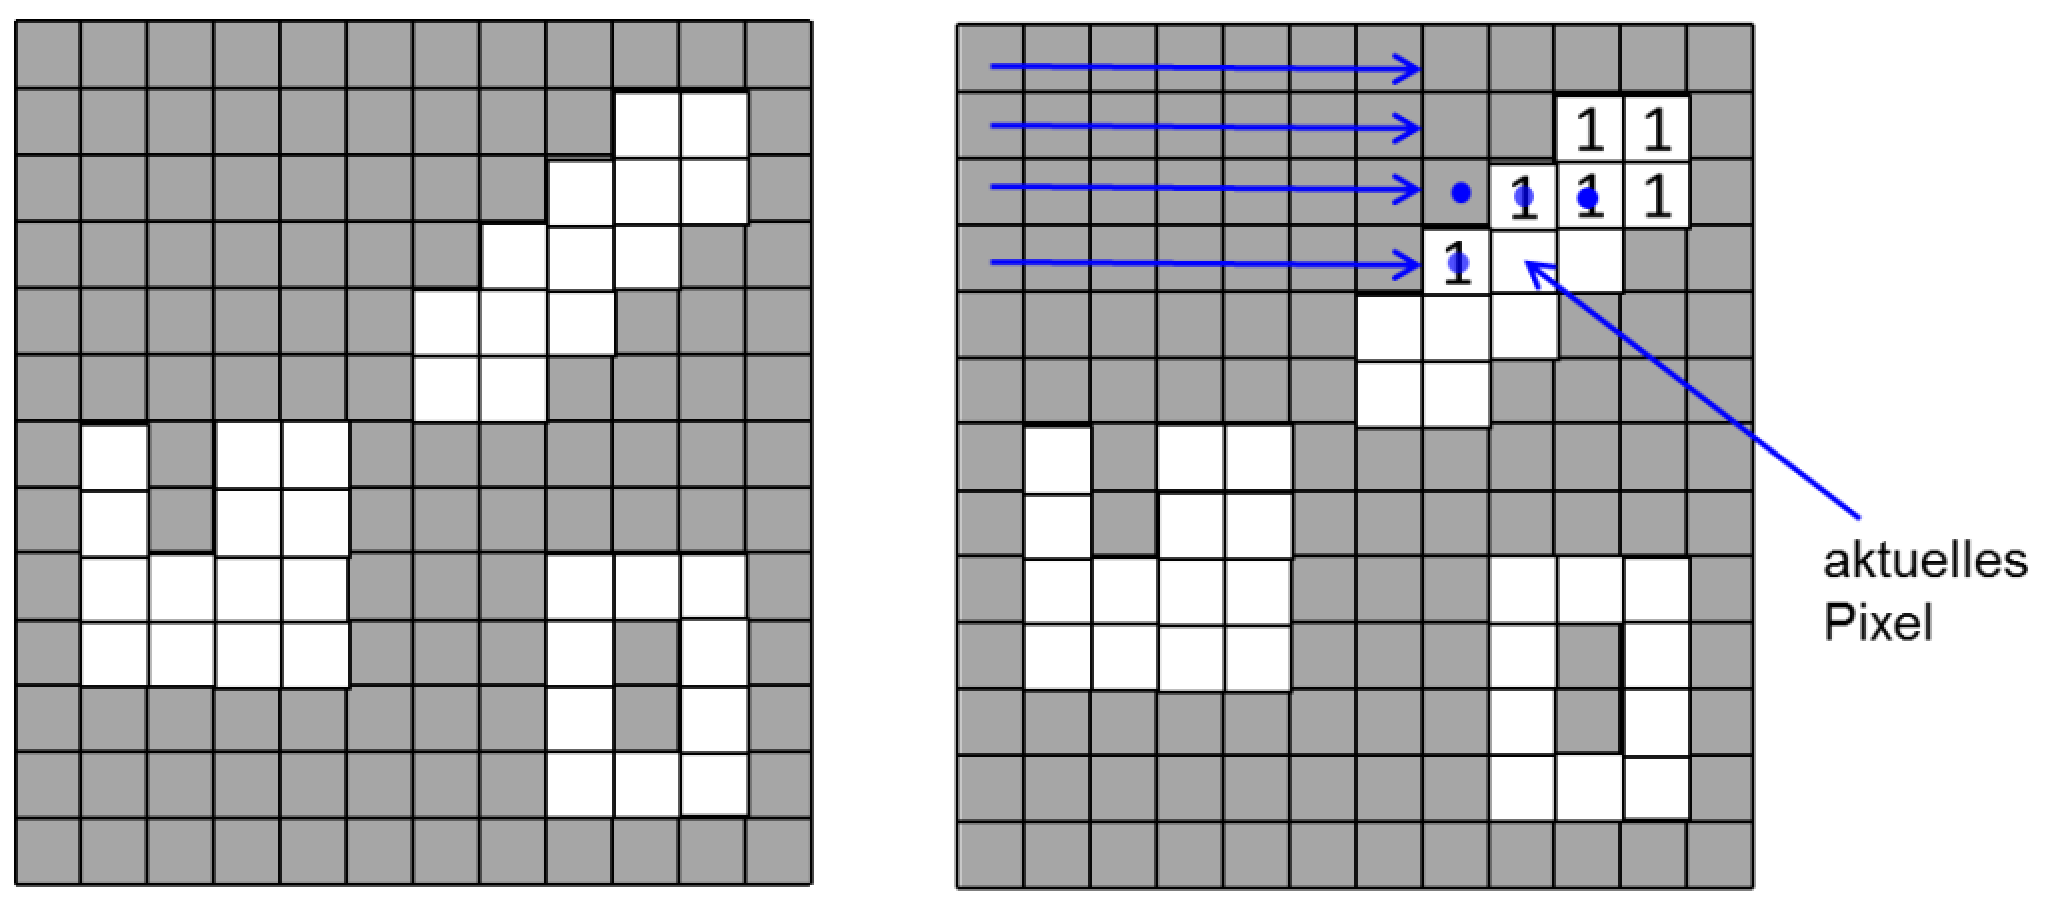
\includegraphics[scale=.5]{../fig/labeling.png}
\end{center}
\begin{center}
	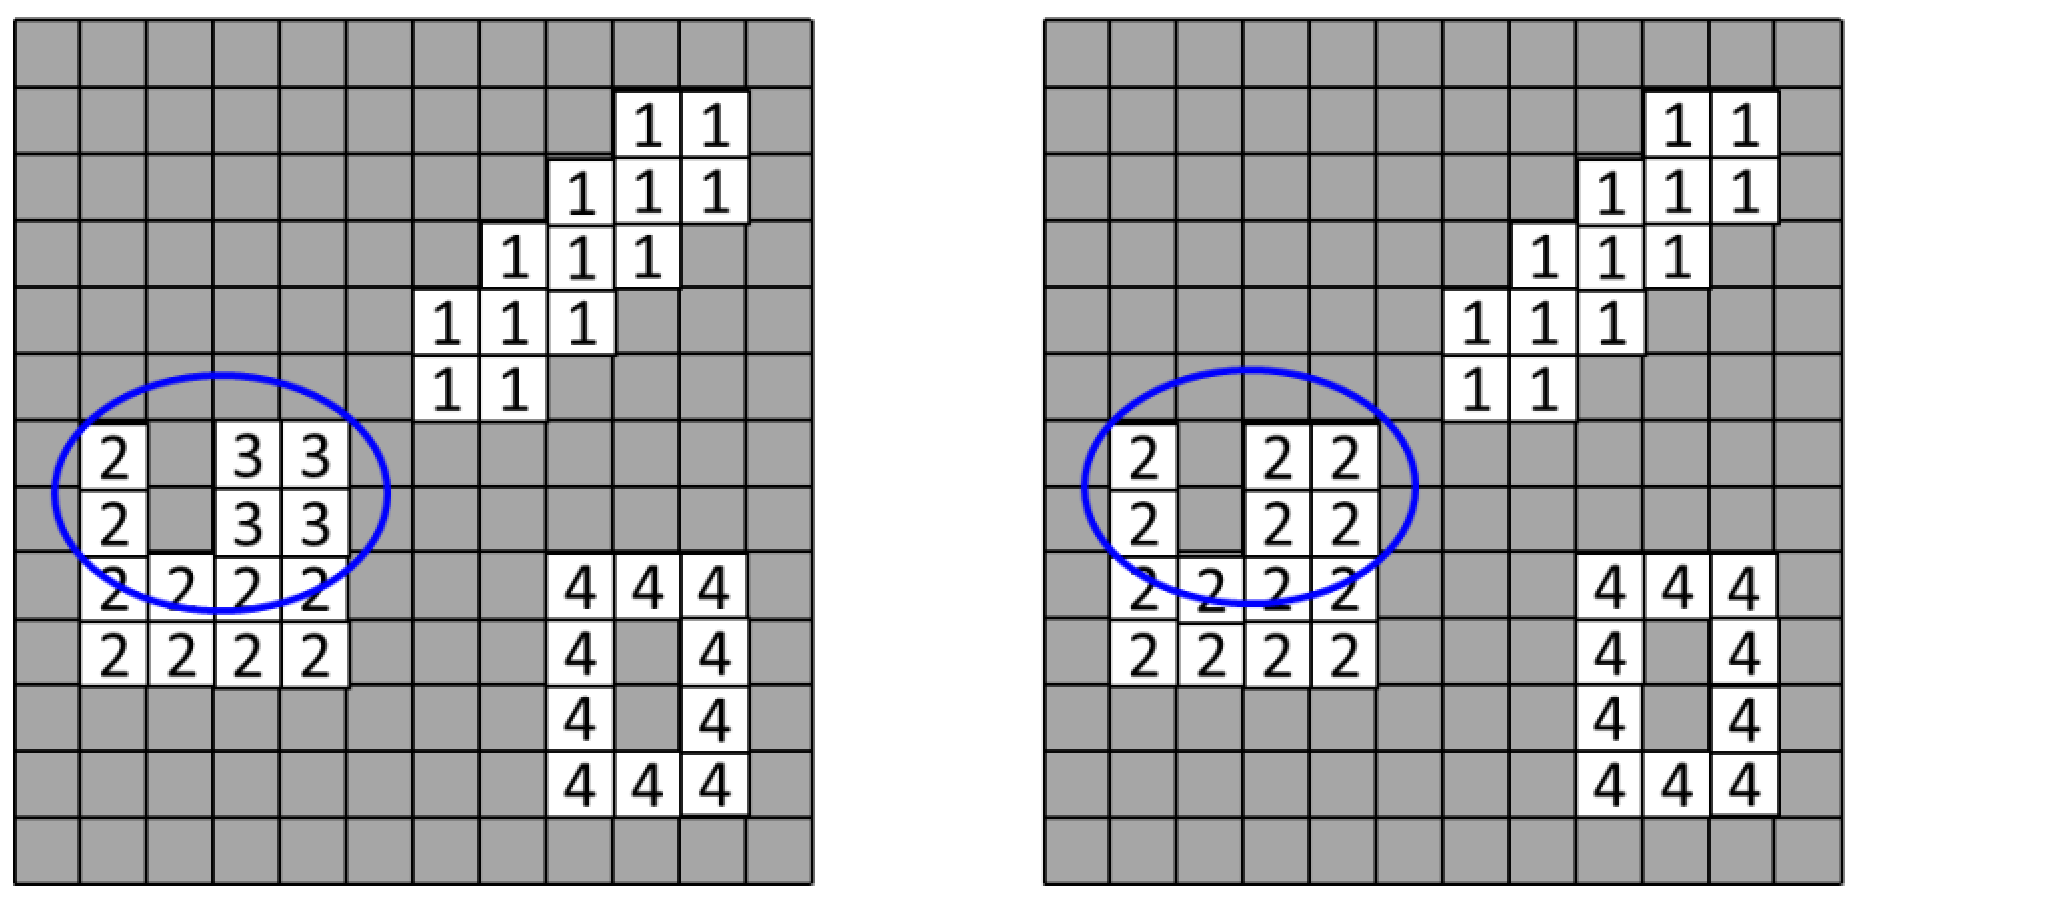
\includegraphics[scale=.5]{../fig/labeling2.png}
\end{center}

\subsection{Kettencode}
Da das Region Labeling häufig einen relativ grossen Speicherbedarft hat, werden in der Regel Kettencodes zur Beschreibung von ROIs verwendet.\\
Die Idee ist, die Randpixel einer ROI, 
ausgehen von einem definierten Startpunkt, 
in sukzessiver Folge nur durch die jeweilige Schrittrichtung vom letzten zum aktuellen Randpixel zu definieren.
\begin{center}
	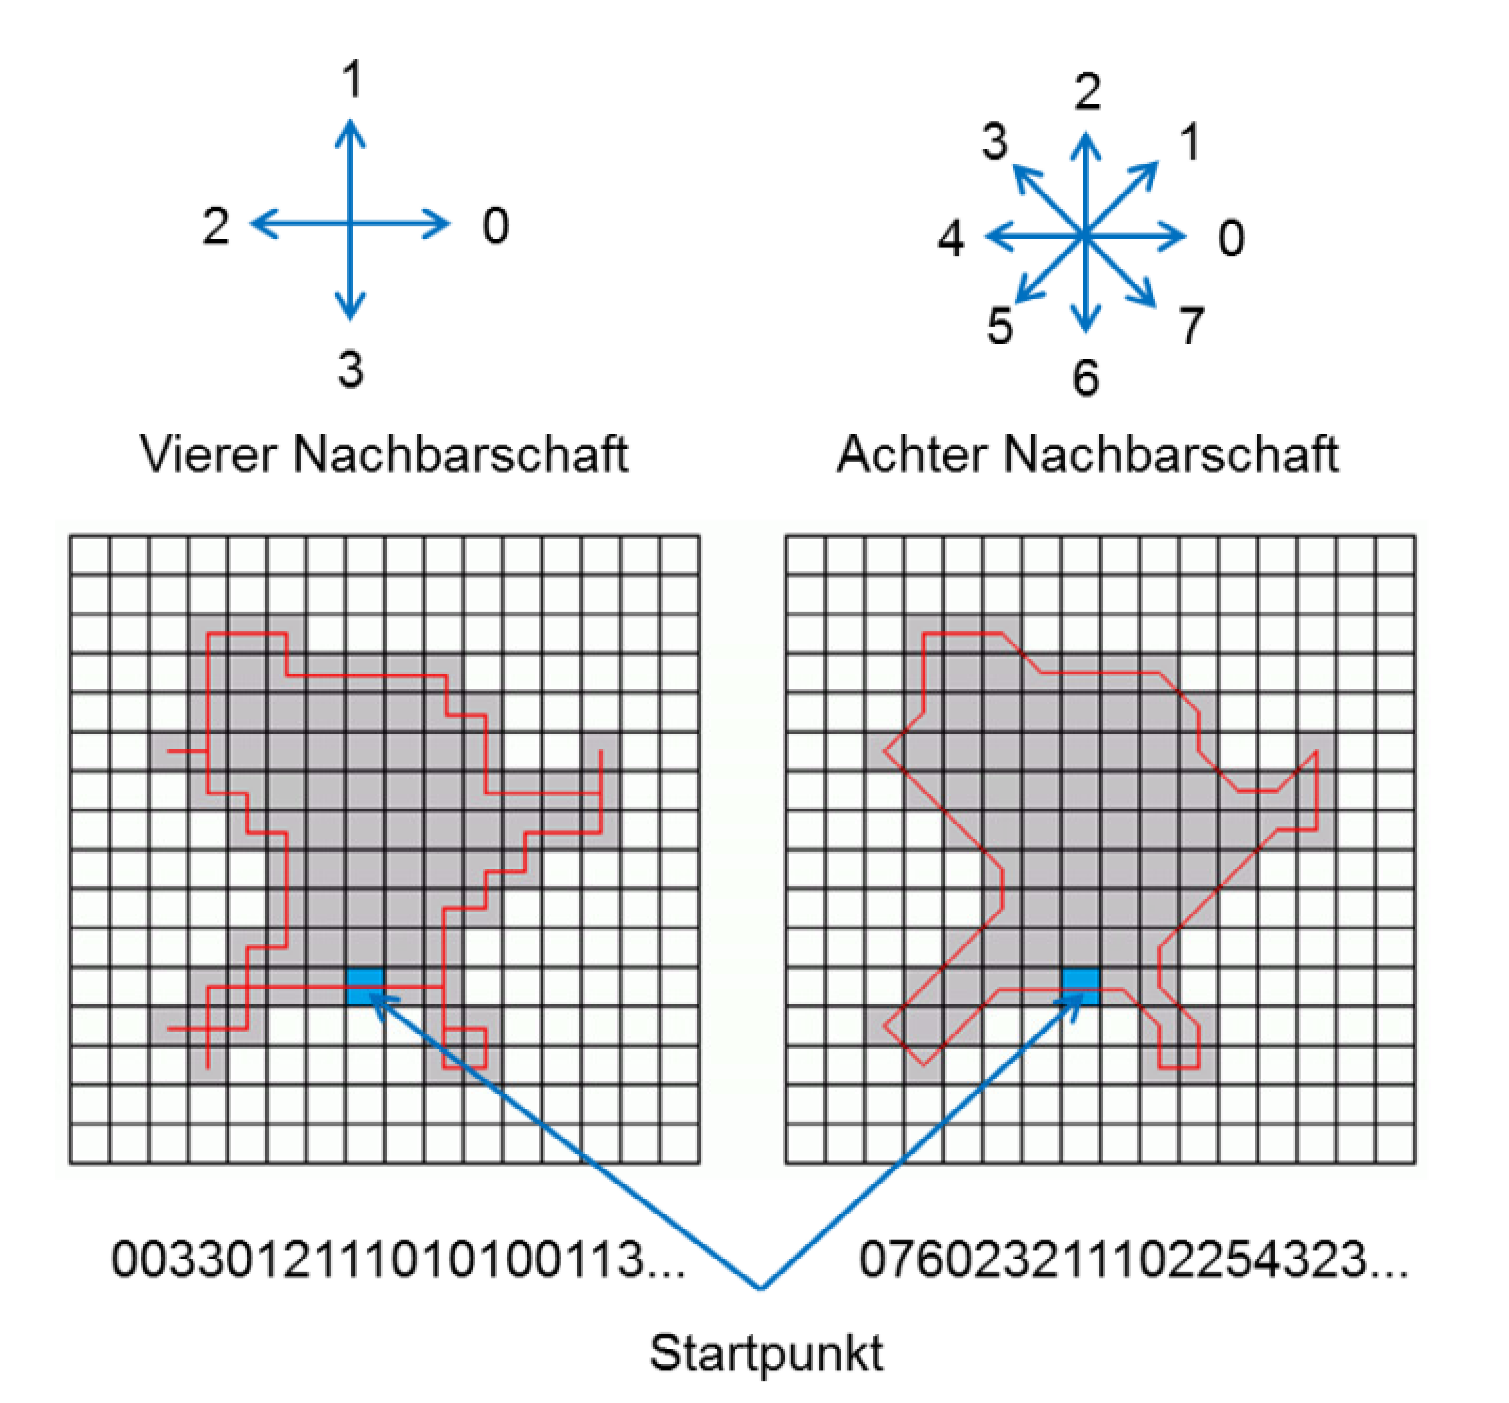
\includegraphics[scale=.5]{../fig/kettencode.png}
\end{center}

\section{Merkmalsextraktion}
Basierend auf der Beschreibung der ROIs mittels Region Labels oder Kettencodes können nun einfach verschiedene ROI Merkmale extrahiert werden.\\
\\
\paragraph{Fläche der ROI:}
\[
	A = \sum_{I_{mn} \in ROI}1
\]
Berechnung anhand von Kettencodes mit dem Crack Code (stellt die Trennlinie zwischen Vorder- und Hintergrund dar):
\[
	A = -\oint_{Rand}y(x)\di x = \sum_{I_{mn} \in \{2-Seg.\}}m - \sum_{I_{mn} \in \{0-Seg.\}}m 
\]
~\\\\
\paragraph{Massnemittelpunkt der ROI:}
\[
	x_s = \frac{1}{A} \sum_{I_{mn}\in ROI}n \qquad y_s = \frac{1}{A} \sum_{I_{mn}\in ROI}m
\]
~\\\\
\paragraph{Umfang der ROI:\\}
Im Falles einer Crack Code basierten Beschreibung der ROIs ist der Umfang einfach durch die Anzahl der Segmente des Codes geben.\\
\\
\paragraph{Orientierung der ROI:\\}
Die Orientierung einer ROI ist definiert als der Winkel zwischen der x-Achse und der längeren der beiden Halbachsen der ROI.
Dabei sind die Halbachsen bestimmt durch die Eigenvektoren der symmetrischen Matrix bestehend aus den zweiten Momenten $M_{xy}$  der ROI:
\begin{scriptsize}\[\begin{aligned}
	M &= \left[\begin{matrix}
	 M_{xx} & M_{xy}\\
	 M_{xy} & M_{yy}\\
	\end{matrix}\right]\\\\
	M_{xx} = \frac{1}{A}\sum_{I_{mn}\in ROI}n^2-{x_s}^2& \qquad
	M_{yy} = \frac{1}{A}\sum_{I_{mn}\in ROI}m^2-{y_s}^2 \\
	M_{xy} &= \frac{1}{A}\sum_{I_{mn}\in ROI}n \cdot m-x_s \cdot y_s
\end{aligned}\]\end{scriptsize}
~\\\\
\paragraph{Bounding Box\\}
Dies ist das kleinste Rechteck, das die ROI noch ganz umschliesst. 
Es ist vor allem nützlich, um schnell Tests bezüglich von Einflussregionen durchzuführen.

~\\\\
Lösung in MATLAB:
\lstset{language=Matlab}
\lstinputlisting[firstline=1,caption=]{../Matlab/MerkmalsExtraktion.m}
~\\
